%============================================================================%
%
%	DOCUMENT DEFINITION
%
%============================================================================%

%we use article class because we want to fully customize the page and dont use a cv template
\documentclass[11pt,A4]{article}


%----------------------------------------------------------------------------------------
%	ENCODING
%----------------------------------------------------------------------------------------

%we use utf8 since we want to build from any machine
\usepackage[polish]{babel}
\usepackage[utf8]{inputenc}

%----------------------------------------------------------------------------------------
%	LOGIC
%----------------------------------------------------------------------------------------

% provides \isempty test
\usepackage{xifthen}

%----------------------------------------------------------------------------------------
%	FONT
%----------------------------------------------------------------------------------------

\usepackage{helvet}

% set font default
\renewcommand*\familydefault{\sfdefault} 	
\usepackage[T1]{fontenc}

% more font size definitions
\usepackage{moresize}		

\usepackage{fontawesome}
\usepackage{worldflags}
%----------------------------------------------------------------------------------------
%	PAGE LAYOUT  DEFINITIONS
%----------------------------------------------------------------------------------------

%debug page outer frames
%\usepackage{showframe}			


%define page styles using geometry
\usepackage[a4paper]{geometry}		

% for example, change the margins to 2 inches all round
\geometry{top=1cm, bottom=-.6cm, left=0.4cm, right=1cm} 	


%less space between header and content
\setlength{\headheight}{-5pt}		


%customize entries left, center and right
%\lhead{}
%\chead{ \small{Jan Küster  $\cdot$ Consultant and Software Engineer $\cdot$  Bremen, Germany  $\cdot$  \textcolor{sectcol}{\textbf{info@jankuester.com}}  $\cdot$ +49 176 313 *** **}}
%\rhead{}


%indentation is zero
\setlength{\parindent}{0mm}

%----------------------------------------------------------------------------------------
%	TABLE /ARRAY DEFINITIONS
%---------------------------------------------------------------------------------------- 

%for layouting tables
\usepackage{multicol}			
\usepackage{multirow}

%extended aligning of tabular cells
\usepackage{array}

\newcolumntype{x}[1]{%
>{\raggedleft\hspace{0pt}}p{#1}}%


%----------------------------------------------------------------------------------------
%	GRAPHICS DEFINITIONS
%---------------------------------------------------------------------------------------- 

%for header image
\usepackage{graphicx}

%for floating figures
\usepackage{wrapfig}
\usepackage{float}
%\floatstyle{boxed} 
%\restylefloat{figure}

%for drawing graphics		
\usepackage{tikz,calc}
\usetikzlibrary{shapes, backgrounds,mindmap, trees}


%----------------------------------------------------------------------------------------
%	Color DEFINITIONS
%---------------------------------------------------------------------------------------- 
\usepackage{transparent}
\usepackage{color}

%accent color
\definecolor{complcol}{RGB}{178,56,80} %stars
\definecolor{emptystar}{RGB}{192, 192, 192}

%dark background color
\definecolor{bgcol}{RGB}{94, 143, 201} % footer and header

%light background / accent color
\definecolor{softcol}{RGB}{133,144,170} %previously: {225,225,225}

\definecolor{sectcol}{RGB}{204, 195, 163} %cvevent background

\definecolor{sidebarcol}{RGB}{133,144,170} %sidebar color


%Package for links, must be the last package used
\usepackage[hidelinks]{hyperref}

%============================================================================%
%
%
%	DEFINITIONS
%
%
%============================================================================%

% returns minipage width minus two times \fboxsep
% to keep padding included in width calculations
\newcommand{\mpwidth}{\linewidth-\fboxsep-\fboxsep}
	

%----------------------------------------------------------------------------------------
% 	TIMELINE
%----------------------------------------------------------------------------------------
\newcommand\ytl[5]{
\parbox[b]{8em}{\hfill{\color{bgcol}\bfseries\sffamily #1}~$\cdots\cdots$~}\makebox[0pt][c]{$\bullet$}\vrule\quad \worldflag[width=0.35cm,length=0.5cm]{#5}\parbox[c]{12cm}{\vspace{7pt}\color{black}\raggedright\sffamily #2: #3 \\ \color{complcol}#4\\[7pt]}\\[-3pt]}

%----------------------------------------------------------------------------------------
% 	ARROW GRAPHICS in Tikz
%----------------------------------------------------------------------------------------

% a six pointed arrow poiting to the left
\newcommand{\tzlarrow}{(0,0) -- (0.2,0) -- (0.3,0.2) -- (0.2,0.4) -- (0,0.4) -- (0.1,0.2) -- cycle;}	

% include the left arrow into a tikz picture
% param1: fill color
%
\newcommand{\larrow}[1]
{\begin{tikzpicture}[scale=0.58]
	 \filldraw[fill=#1!100,draw=#1!100!black]  \tzlarrow
 \end{tikzpicture}
}

% a six pointed arrow poiting to the right
\newcommand{\tzrarrow}{ (0,0.2) -- (0.1,0) -- (0.3,0) -- (0.2,0.2) -- (0.3,0.4) -- (0.1,0.4) -- cycle;}

% include the right arrow into a tikz picture
% param1: fill color
%
\newcommand{\rarrow}
{\begin{tikzpicture}[scale=0.7]
	\filldraw[fill=sectcol!100,draw=sectcol!100!black] \tzrarrow
 \end{tikzpicture}
}

%----------------------------------------------------------------------------------------
%	custom sections
%----------------------------------------------------------------------------------------

% create a coloured box with arrow and title as cv section headline
% param 1: section title
%
\newcommand{\cvsection}[1]
{
\colorbox{sectcol}{\mystrut \makebox[1\mpwidth][l]{
\larrow{bgcol} \hspace{-8pt} \larrow{bgcol} \hspace{-8pt} \larrow{bgcol} \textbf{\textcolor{white}{\uppercase{#1}}}
}}
}

% create a coloured arrow with title as cv meta section section
% param 1: meta section title
%
\newenvironment{metasection}[1] {
	\vspace{6pt}
	\begin{center}
		\textcolor{white}{\large{\uppercase{#1}}}\\
	\normalsize
	\parbox{0.7\mpwidth}{\textcolor{white}	\hrule}
}{\end{center}}

%----------------------------------------------------------------------------------------
%	 PERCENTAGE CIRCLE
%----------------------------------------------------------------------------------------
\newlength\charwidth
\newlength\chwidth
\newcommand*\circled[1]%
  \settototalheight\chwidth{#1\,\%}%
  \ifdim\chwidth>\charwidth\let\charwidth\chwidth\fi
  \addtolength\charwidth{5pt}% twice inner sep plus half line width
  \tikz[baseline=(char.base)];
    \draw [line width=2pt, color=complcol] (char.north) arc (90:90-#1*3.6:.5\charwidth) coordinate (a);
    \draw [line width=2pt, color=sidebarcol]  (a) arc (90-#1*3.6:-270:.5\charwidth);
  }%
}

%----------------------------------------------------------------------------------------
%	 CV ICON
%----------------------------------------------------------------------------------------
\newcommand{\cvicon}[1]
{
    \includegraphics[width={0.07}\mpwidth]{#1}
}

%----------------------------------------------------------------------------------------
%	 CV SCHOOL
%----------------------------------------------------------------------------------------

% creates a stretched box as cv entry headline followed by two paragraphs about
% the work you did
% param 1:	event time i.e. 2014 or 2011-2014 etc.
% param 2:	event name (what did you do?)
% param 3:	institution (where did you work / study)
% param 4:	what was your position
% param 5:	some words about your contributions
%
\newcommand{\cvschool}[5]
{
\vspace{1pt}
	\begin{tabular*}{1\mpwidth}{p{0.55\mpwidth}  x{0.42\mpwidth}}
 	\textcolor{black}{\textbf{#2}} & \textcolor{complcol}{#3}, \textcolor{bgcol}{#1}

	\end{tabular*}
\vspace{-12pt}
\textcolor{softcol}{\hrule}
\vspace{6pt}
	\begin{tabular*}{0.5\mpwidth}{p{\mpwidth}}
\larrow{softcol}  #4\\[3pt]
\larrow{softcol}  #5\\[6pt]
	\end{tabular*}

}

%----------------------------------------------------------------------------------------
%	 CV EVENT
%----------------------------------------------------------------------------------------

% creates a stretched box as cv entry headline followed by two paragraphs about 
% the work you did
% param 1:	event time i.e. 2014 or 2011-2014 etc.
% param 2:	event name (what did you do?)
% param 3:	institution (where did you work / study)
% param 4:	what was your position
% param 5:	some words about your contributions
%
\newcommand{\cvevent}[5]
{
\vspace{1pt}
	\begin{tabular*}{1\mpwidth}{p{0.37\mpwidth}  x{0.60\mpwidth}}
 	\textcolor{black}{\textbf{#2}} & \textcolor{complcol}{#3}, \textcolor{bgcol}{#1} 

	\end{tabular*}
\vspace{-12pt}
\textcolor{softcol}{\hrule}
\vspace{6pt}
	\begin{tabular*}{0.5\mpwidth}{p{\mpwidth}}
\larrow{softcol}  #4\\[3pt]
\larrow{softcol}  #5\\[6pt]
	\end{tabular*}

}

%----------------------------------------------------------------------------------------
%	 PORTFOLIO ITEM
%----------------------------------------------------------------------------------------

\newcommand{\portfolioitem}[8]
{
\medskip
\vspace{1pt}
	\begin{tabular*}{1\mpwidth}{p{0.42\mpwidth}  x{0.55\mpwidth}}
 	\textcolor{black}{\textbf{#2}} & \textcolor{complcol}{#3}, \textcolor{bgcol}{#1}

	\end{tabular*}
\vspace{-12pt}
\textcolor{softcol}{\hrule}
\vspace{5pt}
  \begin{tabular}{ c m{13cm} }
    \begin{minipage}{.3\textwidth}
         \textcolor{white}{#8}\includegraphics[width={#5}\mpwidth]{#4}
    \end{minipage}
    & #6

Related links: #7 \\
  \end{tabular}
}

\newcommand{\portfoliohref}[2]{
\href[pdfnewwindow=true]{#1}{\color{complcol}{#2}}
}

%----------------------------------------------------------------------------------------
%	 CV EVENT LONG
%----------------------------------------------------------------------------------------

% creates a stretched box as cv entry headline followed by two paragraphs about
% the work you did
% param 1:	event time i.e. 2014 or 2011-2014 etc.
% param 2:	event name (what did you do?)
% param 3:	institution (where did you work / study)
% param 4:	what was your position
% param 5:	some words about your contributions
% param 6:	some words about your contributions
% param 7:	some words about your contributions
%
\newcommand{\cveventlong}[7]
{
\vspace{1pt}
	\begin{tabular*}{1\mpwidth}{p{0.40\mpwidth}  x{0.57\mpwidth}}
 	\textcolor{black}{\textbf{#2}} & \textcolor{complcol}{#3}, \textcolor{bgcol}{#1}

	\end{tabular*}
\vspace{-12pt}
\textcolor{softcol}{\hrule}
\vspace{6pt}
	\begin{tabular*}{0.5\mpwidth}{p{\mpwidth}}
\larrow{softcol}  #4\\[3pt]
\larrow{softcol}  #5\\[6pt]
\larrow{softcol}  #6\\[6pt]
\larrow{softcol}  #7\\[6pt]
	\end{tabular*}

}

%----------------------------------------------------------------------------------------
%	 CV EVENT ONE
%----------------------------------------------------------------------------------------

% creates a stretched box as cv entry headline followed by two paragraphs about
% the work you did
% param 1:	event time i.e. 2014 or 2011-2014 etc.
% param 2:	event name (what did you do?)
% param 3:	institution (where did you work / study)
% param 4:	what was your position
%
\newcommand{\cveventone}[4]
{
\vspace{1pt}
	\begin{tabular*}{1\mpwidth}{p{0.55\mpwidth}  x{0.42\mpwidth}}
 	\textcolor{black}{\textbf{#2}} & \textcolor{complcol}{#3}, \textcolor{bgcol}{#1}

	\end{tabular*}
\vspace{-12pt}
\textcolor{softcol}{\hrule}
\vspace{6pt}
	\begin{tabular*}{0.5\mpwidth}{p{\mpwidth}}
\larrow{softcol}  #4\\[3pt]
	\end{tabular*}

}

%----------------------------------------------------------------------------------------
%	 SIMPLE LIST
%----------------------------------------------------------------------------------------

% creates a stretched box as cv entry headline followed by two paragraphs about
% the work you did
% param 1:	List title
% param 2:	First line
% param 3:	2nd line
%
\newcommand{\simplelist}[3]
{
\vspace{1pt}
	\begin{tabular*}{1\mpwidth}{p{0.48\mpwidth}  x{0.49\mpwidth}}
 	\textcolor{black}{\textbf{#1}}

	\end{tabular*}
\vspace{-12pt}
\textcolor{softcol}{\hrule}
\vspace{6pt}
	\begin{tabular*}{0.5\mpwidth}{p{\mpwidth}}
\larrow{softcol}  #2\\[3pt]
\larrow{softcol}  #3\\[3pt]
	\end{tabular*}

}

% creates a stretched box as 
\newcommand{\cveventmeta}[2]
{
	\mbox{\mystrut \hspace{87pt}\textit{#1}}\\
	#2
}

%----------------------------------------------------------------------------------------
% CUSTOM STRUT FOR EMPTY BOXES
%----------------------------------------- -----------------------------------------------
\newcommand{\mystrut}{\rule[-.3\baselineskip]{0pt}{\baselineskip}}

%----------------------------------------------------------------------------------------
% CUSTOM LOREM IPSUM
%----------------------------------------------------------------------------------------
\newcommand{\lorem}
{Lorem ipsum dolor sit amet, consectetur adipiscing elit. Donec a diam lectus.}


% use to vertically center content
% credits to: http://tex.stackexchange.com/questions/7219/how-to-vertically-center-two-images-next-to-each-other
\newcommand{\vcenteredinclude}[1]{\begingroup
\setbox0=\hbox{\includegraphics{#1}}%
\parbox{\wd0}{\box0}\endgroup}

% use to vertically center content
% credits to: http://tex.stackexchange.com/questions/7219/how-to-vertically-center-two-images-next-to-each-other
\newcommand*{\vcenteredhbox}[1]{\begingroup
\setbox0=\hbox{#1}\parbox{\wd0}{\box0}\endgroup}

%----------------------------------------------------------------------------------------
%	ICON-SET EMBEDDING
%---------------------------------------------------------------------------------------- 

% at this point we simplify our icon-embedding by simply referring to a set of png images.
% if you find a good way of including svg without conflicting with other packages you can
% replace this part
\newcommand{\icon}[3]{\makebox(#2, #2){\textcolor{#3}{\csname fa#1\endcsname}}}	%icon shortcut
\newcommand{\icontext}[4]{ 						%icon with text shortcut
	\vcenteredhbox{\icon{#1}{#2}{#4}} \vcenteredhbox{\textcolor{#4}{#3}}
}
\newcommand{\iconhref}[5]{ 						%icon with website url
    \vcenteredhbox{\icon{#1}{#2}{#5}} \href{#4}{\textcolor{#5}{#3}}
}

\newcommand{\iconemail}[5]{ 						%icon with email link
    \vcenteredhbox{\icon{#1}{#2}{#5}} \href{mailto:#4}{\textcolor{#5}{#3}}
}



%============================================================================%
%
%
%
%	DOCUMENT CONTENT
%
%
%
%============================================================================%
\begin{document}
\fcolorbox{white}{white}{\begin{minipage}[c][0.97\textheight][t]{0.72\linewidth}


%---------------------------------------------------------------------------------------
%	TITLE HEADLINE
%----------------------------------------------------------------------------------------
\vspace{-3pt}
% use this for multiple words like working titles etc.
%\hspace{-0.25\linewidth}\colorbox{bgcol}{\makebox[1.5\linewidth][c]{\hspace{46pt}\HUGE{\textcolor{white}{\uppercase{M.Sc. Jan Küster}} } \textcolor{sectcol}{\rule[-1mm]{1mm}{0.9cm}} \parbox[b]{5cm}{   \large{ \textcolor{white}{{IT Consultant}}}\\
% \large{ \textcolor{white}{{JS Fullstack Engineer}}}}
%}}

% use this for single words, e.g. CV or RESUME etc.
\colorbox{bgcol}{\makebox[\mpwidth][c]{\textcolor{white}{\HUGE{Michał Żyłowski}}\HUGE{\textcolor{white}{\uppercase{ CV}} } }}

%----------------------------------------------------------------------------------------
%	HEADER IMAGE
%----------------------------------------------------------------------------------------


%\hspace{-1.6cm}
%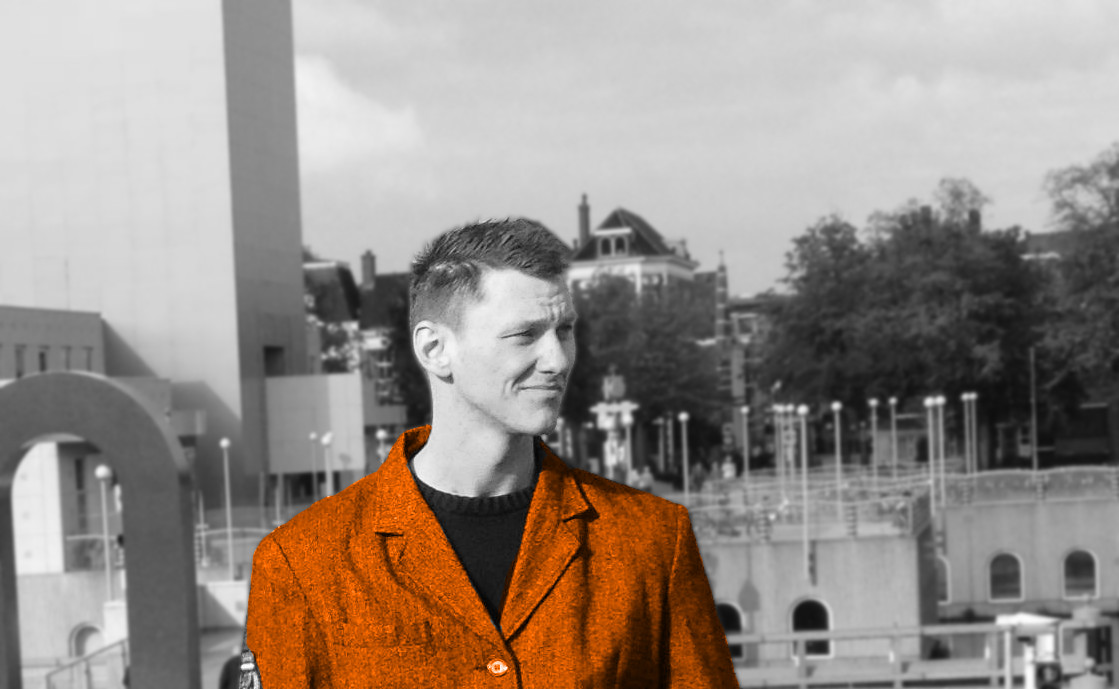
\includegraphics[trim= 0 250 0 270,clip,width=1\linewidth+3.1cm]{myfoto.jpg}	%trimming relative to image size!
%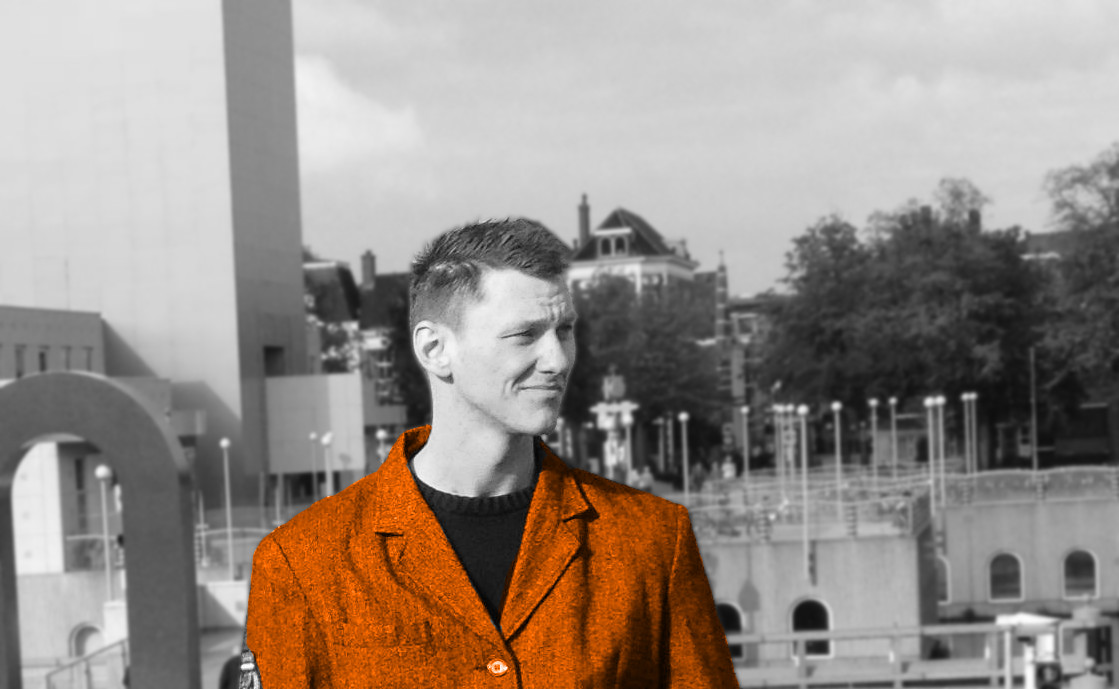
\includegraphics[trim= 350 150 0 200, clip ,width=\linewidth]{myfoto.jpg}	%trimming relative to image size

%---------------------------------------------------------------------------------------
%	SUMMARY
%----------------------------------------------------------------------------------------
%\transparent{0.85}%
%\vspace{-130pt}
%\hspace{0.4\linewidth}
%\colorbox{bgcol}{
%	\parbox{0.5\linewidth}{
%		\transparent{1}%
%		\begin{center}
%		\larrow{sectcol}\larrow{sectcol}\textcolor{white}{I create awesome resume templates in LaTeX for everyone. Besides that I am working at the University of Bremen and engineer fullstack JS applications with Meteor.}
%		\end{center}
%	}
%}
%\vspace{60pt}

%============================================================================%
%
%	CV SECTIONS AND EVENTS (MAIN CONTENT)
%
%============================================================================%

%---------------------------------------------------------------------------------------
%	STATUS
%----------------------------------------------------------------------------------------
\cvsection{Status}\\[5pt]
Senior DevOps engineer working at Dynatrace on robust deployment tool called DoK (Dynatrace on Kubernetes). This tool can deploy fully working AKS/GKE cluster and will push there multiple needed helm apps. I'm responsible for my code change on all levels: from terraform/python/bash code, through review and merging, up to prodding new packages to the production environment. Believer of open source philosophy. The breadth of knowledge approach.
\vspace{5pt}

%---------------------------------------------------------------------------------------
%	EXPERIENCE
%----------------------------------------------------------------------------------------
\cvsection{EMPLOYMENT HISTORY}

%
\cvevent{2022/10 - now}{Dynatrace}{Senior Cloud DevOps}{Dynatrace on Kubernetes project team member, responsible for deploying end product app on Azure and Google clouds.}{Maintainer of multiple production k8s clusters with huge number of resources.}
\cvevent{2020/05 - 2022/10}{OVHcloud}{Cloud DevOps}{OVH public cloud R\&D team member, responsible for networking in OpenStack.}{OVH Public Cloud expert. Workshops and conferences speaker.}
\cvevent{2018/09 - 2021/06}{Gdańsk WSB University}{Lecturer}{Teacher of programming languages like: Python, C++, Java, C\#.} {Tutor of concepts like: Cloud, OOP, WWW designing, Version Control.}
\cveventlong{2015/05 - 2020/05}{Intel Technology Poland}{Programmer \& DevOps}{2018/11 Software Cloud Engineer at Artificial Intelligence group in Nauta project.}{2017/10 Software Development Engineer at Linux Virtual RAID on CPU project.}{2017/05 Software Validation Engineer at Rapid Storage Technology enterprise team.}{2015/05 Software Engineer Intern at Software Defined Infrastructure team.}

%\textcolor{softcol}{\hrule}

\vspace{5pt}
%---------------------------------------------------------------------------------------
%	EDUCATION
%--------------------------------------------------------------------------------------
\cvsection{EDUCATION}

\cvschool{2012-2017}{Gdańsk University of Technology}{ETI Faculty}{Master degree: Informatics, full-time. Thesis: Mesos schedulers examination.}{Engineering degree: Informatics, full-time. Thesis: Programmable RTS game.}
\cveventone{2007-2011}{Zespół Szkół Technicznych Grudziądz}{IT technical school}{Course: Computer Science, Specialization: Internet Applications.}
\simplelist{Certificates}{2016/07  Linux Troubleshooting training performed by Hewlett Packard Enterprise}{2013/06 “ABC of business management” certificate.}

%---------------------------------------------------------------------------------------
%	TOP SKILLS
%--------------------------------------------------------------------------------------
\cvsection{TOP SKILLS}

\larrow{softcol} Taking part in a software development process using agile methodologies.

%\larrow{softcol} Understanding Test Driven Development technique.

\larrow{softcol} Ability to debug complex and not obvious issues in Linux ecosystems.

%\larrow{softcol} Working using agile methodologies (Scrum, Kanban).

\larrow{softcol} Understanding concept of CI/CD and experience in Argo WF and GH Actions.

\larrow{softcol} Maintaining production k8s clusters in both private and public environments.

\larrow{softcol} Experienced in cooperation and collaboration with open source communities.

\larrow{softcol} Linux kernel building and debugging. I have a small patch in the Linux kernel tree.

\larrow{softcol} Taking care of details and minor issues that affect the quality of the product.

\larrow{softcol} Tenacity during issue fixing and taking responsibility for the result.

\larrow{softcol} Competence to present solutions at conferences or meetings with customers.
\vspace{5px}

\end{minipage}}%
\fcolorbox{white}{sidebarcol}{\begin{minipage}[c][0.97\textheight][t]{0.28\linewidth}


\begin{center}
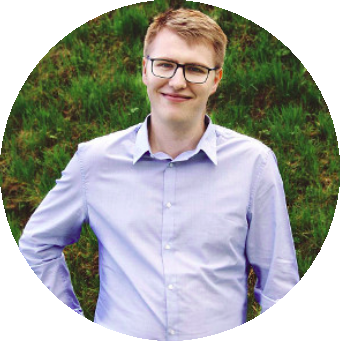
\includegraphics[width=0.7\mpwidth]{img/mz.png}

\icontext{MapMarker}{12}{Gdańsk, Poland}{white}\\[5pt]
\icontext{Calendar}{12}{32 years old}{white}\\[5pt]
\end{center}

\begin{metasection}{Contact}

	\iconhref{MousePointer}{12}{zylowski.net}{https://zylowski.net}{white}\\[5pt]
	\iconhref{Github}{12}{github.com/mzylowski}{https://github.com/mzylowski}{white}\\[5pt]
	\iconhref{Linkedin}{12}{@michal\_zylowski}{https://www.linkedin.com/in/mzylowski}{white}\\[5pt]
%	\icontext{MobilePhone}{12}{+48 *** *** ***}{white}\\[5pt]
	\iconemail{Envelope}{12}{michal@zylowski.net}{michal@zylowski.net}{white}\\[5pt]
\end{metasection}

%----------------------------------------------------------------------------------------
%	META SECTION
%----------------------------------------------------------------------------------------

\begin{metasection}{Fields}

\icontext{Code}{12}{Software Development}{white}\\[5pt]
\icontext{Retweet}{12}{Automation}{white}\\[5pt]
\icontext{Bolt}{12}{Mentoring}{white}\\[5pt]
\icontext{Server}{12}{DevOps}{white}\\[5pt]
\icontext{Cloud}{12}{Cloud}{white}\\[5pt]
\icontext{CheckCircle}{12}{CI/CD}{white}\\[5pt]

\end{metasection}
\begin{metasection}{Tools}

\textcolor{white}{
\icontext{Cubes}{12}{Pycharm}{white} \icontext{Terminal}{12}{Terminal}{white} \\[5pt] \icontext{CodeFork}{12}{Git}{white} \icontext{Tasks}{12}{Jira}{white}\icontext{Github}{12}{Github}{white} \\[5pt] \icontext{Refresh}{12}{k9s}{white} \icontext{Slack}{12}{Slack}{white}\\
}
\end{metasection}

\begin{metasection}{Languages}

\textcolor{white}{
\icontext{Language}{12}{Polish}{white} \icontext{Wechat}{12}{English}{white}
}
\end{metasection}

%\vspace{17pt}

\begin{metasection}{Legal}

\footnotesize\textcolor{white}{
I agree to the processing of personal data provided in this document for realising the recruitment process pursuant to the Personal Data Protection Act of 10 May 2018 (Journal of Laws 2018, item 1000) on the protection of natural persons with regard to the processing of personal data and on the free movement of such data, and repealing Directive 95/46/EC (GDPR).
}
\end{metasection}


%\begin{metasection}{Activities}
%
%\textcolor{white}{\LARGE{\icon{Gamepad}{24}{white} \icon{Headphones}{24}{white}  \icon{Bicycle}{24}{white}}}
%\end{metasection}

%\begin{metasection}{Operating Systems}
%
%\textcolor{white}{\LARGE{\icon{Linux}{24}{white} \icon{Android}{24}{white}  \icon{Windows}{24}{white}}}
%
%\end{metasection}

%---------------------------------------------------------------------------------------
%	END OF SIDEBAR
%----------------------------------------------------------------------------------------

\end{minipage}}

%-------------------------------------------------------------------------------------------------
%	ARTIFICIAL FOOTER (fancy footer cannot exceed linewidth)
%--------------------------------------------------------------------------------------------------

\vspace*{\fill}
\hspace{-0.25\linewidth}\colorbox{bgcol}{\makebox[1.5\linewidth][c]{\mystrut \small \textcolor{white}{ }}}


\newpage

%---------------------------------------------------------------------------------------
%	TOP TECHNOLOGIES
%--------------------------------------------------------------------------------------
\cvsection{MY TECH STACK}

\larrow{softcol} Top technologies:
\begin{center}
\begin{tabular}{ c c c c c c}
\cvicon{img/icons/png/kubernetes.png} & \cvicon{img/icons/png/openstack.png} & \cvicon{img/icons/png/python.png} & \cvicon{img/icons/png/gnubash.png} & \cvicon{img/icons/png/linux.png} & \cvicon{img/icons/png/protonvpn.png}\\[12pt]
Kubernetes & OpenStack & Python & BASH & Linux & Networking \\[12pt]
\end{tabular}
\end{center}

\larrow{softcol} Programming languages that I also touched:
\begin{center}
\begin{tabular}{ c c c c c}
\cvicon{img/icons/png/go.png} & \cvicon{img/icons/png/csharp.png} & \cvicon{img/icons/png/cplusplus.png} & \cvicon{img/icons/png/html5.png} & \cvicon{img/icons/png/mysql.png}\\[12pt]
GO & C\# & C++ & Web Dev & SQL \\[12pt]
\end{tabular}
\end{center}

\larrow{softcol} Cloud providers that I know:
\begin{center}
\begin{tabular}{ c c c c c}
\cvicon{img/icons/png/azuredevops.png} & \cvicon{img/icons/png/googlecloud.png} & \cvicon{img/icons/png/amazonaws.png} & \cvicon{img/icons/png/ovh.png} & \cvicon{img/icons/png/gnometerminal.png}\\[12pt]
Azure & GCP & AWS & OVHcloud & Private Clouds \\[12pt]
\end{tabular}
\end{center}

\larrow{softcol} CI/CD and automation tools:
\begin{center}
\begin{tabular}{ c c c c c c c}
\cvicon{img/icons/png/argo.png} & \cvicon{img/icons/png/jenkins.png} & \cvicon{img/icons/png/githubactions.png} & \cvicon{img/icons/png/circleci.png} & \cvicon{img/icons/png/ansible.png} & \cvicon{img/icons/png/puppet.png} & \cvicon{img/icons/png/terraform.png}\\[12pt]
Argo Workflows & Jenkins & Github Actions & Circle CI & Ansible & Puppet & Terraform \\[12pt]
\end{tabular}
\end{center}

\larrow{softcol} Other tools and areas:
\begin{center}
\begin{tabular}{ c c c c c c}
\cvicon{img/icons/png/vault.png} & \cvicon{img/icons/png/docker.png} & \cvicon{img/icons/png/amazons3.png} & \cvicon{img/icons/png/apache.png} \\[12pt]
Vault & Containers & Minio/S3 & Apache Mesos \\[3pt]
\end{tabular}
\end{center}

%---------------------------------------------------------------------------------------
%	MAJOR TALKS ON CONFERENCES
%--------------------------------------------------------------------------------------
\cvsection{MAJOR TALKS ON CONFERENCES}
\begin{table}[!h]
%\caption{Timeline of talks}
\centering
\begin{minipage}[t]{.7\linewidth}
\color{gray}
\rule{\linewidth}{1pt}
\ytl{25.11.2021}{WARSAW}{Innovation for Freedom}{\portfoliohref{https://github.com/mzylowski/ovh-workshops/tree/main/demo25.11.21}{WORKSHOP: Cloud Means Freedom.}}{GB}
\ytl{23.03.2022}{REMOTE}{Targi pracy Jobicon: Czym jest chmura?}{\portfoliohref{https://raw.githubusercontent.com/mzylowski/mzylowski/master/cv/cv/confs/jobicon22.png}{PRESENTATION: O usługach chmurowych w prostych słowach}}{PL}
\ytl{05-06.2022}{KRAKÓW, KATOWICE, WROCŁAW}{OVH RoadShow}{\portfoliohref{https://www.cloudforum.pl/2022/04/21/ovhcloud-techroadshow-czyli-jak-budowac-nowoczesne-aplikacje-w-europejskiej-chmurze-publicznej/}{WORKSHOP: Chmura publiczna OVHcloud.}}{PL}
\ytl{09.06.2022}{BERLIN}{Open Infrastructure Summit 2022}{\portfoliohref{https://www.youtube.com/watch?v=S9zXMmBlRKE}{TALK: How we integrated L3 services into one of the biggest OpenStack Public Cloud? OVHcloud case study.}}{GB}
\bigskip
\rule{\linewidth}{1pt}%
\end{minipage}%
\end{table}

%---------------------------------------------------------------------------------------
%	HOBBIES
%--------------------------------------------------------------------------------------
\cvsection{HOBBIES}

\larrow{softcol} Geocaching, astronomy, chess, opera, mountains, art exhibitions, smart home.

\vspace*{\fill}
\hspace{-0.25\linewidth}\colorbox{bgcol}{\makebox[1.5\linewidth][c]{\mystrut \small \textcolor{white}{ }}}

\newpage
\cvsection{Projects Portfolio}

\portfolioitem{2022/10 - now}{Dynatrace on Kubernetes}{Developer \& DevOps \& Production maintainer}{img/dynatrace.png}{0.8}
{Dynatrace on Kubernetes (DoK) is a internal tooling - set of terraform code, charts, python and bash scripts, that fully running will deploy working Kubernetes cluster on chosen cloud provider (AWS, Azure, Google). Together with infrastructure deployed by terraform, also applications released by helm charts will be delivered to the cluster. We deploying huge Java application as our Dynatrace server, multiple Cassandra and ElasticSearch pods as backend for the server, ingress and many more smaller applications. Tooling is delivered together with advanced Argo workflows that supports k8s upgrades without downtime, backup, disaster recovery and more. I was implementing multiple features at all levels of this solution, but most significant for me was pushing HashiCorp Vault to DoK stack.}
{\portfoliohref{https://github.com/cscetbon/casskop}{n/a}}{------}

\portfolioitem{2020/05 - 2022/10}{Networking in OVHcloud Public Cloud}{Code developer \& DevOps}{img/ovhcloud.jpg}{1.0}
{OVH's Public Cloud is built on an OpenStack solution, where project Neutron is responsible for the networking part. To handle networking in a way that OVH needs, few python agents (Neutron plugins) were introduced. In R\&D team where I also belong, we are responsible for developing and maintaining those plugins. This includes bug fixing, deep debugging around the Linux system and networking, upgrading to new OpenStack releases and delivering new features like L3 services or virtual routers.}
{\portfoliohref{https://github.com/svinota/pyroute2/pull/779}{Example of external contribution}}{-}

\portfolioitem{2019/07 - 2019/10}{Video training about Kubernetes}{Author \& Tutor}{img/helion.png}{1.0}
{During summer 2019, I prepared video training about Kubernetes orchestrator. Course is available to buy even now on Helion (Polish publishing house) website. The training is available only in the Polish language. The course starts with a complete basis, covers all elementary Kubernetes objects, goes through k8s deployment and in the end it touches a bit more advanced topics like init containers, security context, exposing services outside of the cluster.}
{\portfoliohref{https://helion.pl/ksiazki/kubernetes-kurs-video-wdrazanie-aplikacji-michal-zylowski,vuruap.htm}{My kubernetes training [PL]}}{-}

\portfolioitem{2018/10 - 2020/05}{Nauta Platform}{Code developer \& DevOps}{img/nauta.png}{1.1}
{Nauta is a deep learning platform developed on top of a Kubernetes cluster that allows scheduling artificial intelligence experiments by data-scientists not familiarized with clouds topics. I joined to Nauta development team when the project was in alpha state. My responsibilities were related to maintaining platform build system written in makefile and ansible, preparing user-guide web UI and fixing bugs in Nauta CLI (python). I also was involved in the development of internal CI/CD solution. Nauta is an open source project published on GitHub, written in python, go-lang, JS and others.}
{\portfoliohref{https://github.com/IntelAI/nauta/commit/7efbdac3e9cc4d64afd6b6e6fb0481e2b2436ff9}{UI component} | \portfoliohref{https://github.com/IntelAI/nauta/commit/c4ecc8a44ba212516ec4dd2f9a4bf830ed589701}{Build system change} | \portfoliohref{https://github.com/IntelAI/nauta/commit/abde914c1eccf2612774e67646564a2f61caa44e}{Nauta CLI change}}{}

\portfolioitem{2017/06 - 2018/10}{Virtual RAID on CPU for Linux}{Developer, External contributor, Maintainer}{img/vroc.jpg}{1.0}
{VROC is a name for the entire solution related with software RAID arrays targeted to enterprise solutions. Solution consists of two Linux applications: mdadm and ledmon, and with kernel module named md. All related code is written in C. My team was responsible for maintenance of IMSM metadata in mdadm and the entire Linux ecosystem. Mdadm is used as CLI tool in RHEL, SLES and Ubuntu operating systems. My work was mostly related with bug fixing and cooperation with operating systems vendors (like SUSE or Cannonical). When mdadm is external kernel project, ledmon is an open source project fully developed by Intel and I was a maintainer of the project and repository. Ledmon was designed for blinking LEDs of disks under RAID arrays in the VROC stack.}
{\portfoliohref{https://github.com/intel/ledmon/commits?author=mzylowski}{My ledmon commits} | \portfoliohref{https://git.kernel.org/pub/scm/linux/kernel/git/torvalds/linux.git/commit/scripts/checkpatch.pl?id=6ad724e2a48fc24dd9788490d85a3490cb0117c1}{Kernel patch} | \portfoliohref{https://git.kernel.org/pub/scm/utils/mdadm/mdadm.git/log/?qt=grep\&q=Michal+Zylowski}{My mdadm patches}}{}

\vspace*{\fill}
\hspace{-0.25\linewidth}\colorbox{bgcol}{\makebox[1.5\linewidth][c]{\mystrut \small \textcolor{white}{ }}}

\newpage

\portfolioitem{2017/02 - 2017/05}{POC and tech analysis: CRI-o with K8S}{Code developer, DevOps}{img/crio-logo.png}{1}
{With a friend from my team I tried to change k8s backend from docker to cri-o. We found some issues to fix on the cri-o part. After merging PR’s related with them, I run e2e k8s conformance tests, to check how many features must be fixed and re-implemented in cri-o. During this POC cri-o was in an early stage and a lot of hacks was required to achieve the goal.}
{\portfoliohref{https://github.com/cri-o/cri-o/pull/342}{Example of contribution} | \portfoliohref{https://github.com/cri-o/cri-o/pull/353}{Result of the POC}}{}

\portfolioitem{2016/05 - 2016/09}{Benchmarking of rkt container system}{Code developer, CI/CD owner}{img/rkt.png}{0.9}
{Rkt is alternative for docker containers. Rkt-monitor is simple golang app included in rkt repo, designed for measuring performance of entire stack. I made some fixes for rkt-monitor and I discovered performance issue. Also I prepared CI solution (based on Jenkins and my own python scripts) for  running measurements daily.}
{\portfoliohref{https://github.com/rkt/rkt/pull/3093/files}{Example of contribution} | \portfoliohref{https://github.com/rkt/rkt/issues/3019}{Discovered issue}}{}

\portfolioitem{2016/10 - 2017/01}{k8s e2e testing \& deployment by Kubespray}{Code developer, DevOps}{img/k8s.png}{0.8}
{Kubespray is a set of ansible scripts related with installing Kubernetes. My team was interested running kubernetes e2e tests with docker and rkt containerizers on bare metal. We were responsible for solving issues and tests in kubernetes one by one. It was important for us to redeploy k8s clusters easy and fast, so I was also involved in kubespray development.}
{\portfoliohref{https://github.com/kubernetes-sigs/kubespray/pull/852}{PR to Kubespray} | \portfoliohref{https://github.com/kubernetes-sigs/kubespray/issues/610}{Issue submitted to Kubespray} | \portfoliohref{https://github.com/kubernetes/kubernetes/pull/35302}{k8s e2e test fix}}{-----}

\portfolioitem{2015/11 - 2016/09}{Serenity (plugin for Mesos)}{Tester}{img/mesos.png}{0.8}
{Serenity is a plugin for Mesos solution. Plugin improves scheduler and resources utilization mechanism. I was responsible for creating check that simulate real user network traffic. Technology stack: Stressing Wikimedia (deployed on Mesos cluster) by the gatling stress tool. Also in this project I helped to decrease time needed to run Mesos oversubscription tests by preparing scripts (ansible + python) for automated tests execution and results collection.}
{\portfoliohref{https://github.com/mesosphere/serenity}{Serenity on github}}{------}

\cvsection{Non profit projects}

\portfolioitem{2017/10 - 2019/06}{New technologies for Women}{Mentor}{img/ntdd.png}{0.8}
{'Perspektywy' foundation and Intel Technology Poland prepared a scholarship program for young women. According to the idea of the project, each scholarship holder receives mentorship support during a one-year scholarship. I was one of 25 mentors from Intel company in 2017/2018 and 2018/2019 editions and I finished this program with two girls.}
{\portfoliohref{https://www.stypendiadladziewczyn.pl/pl/o-programie}{Scholarship program site}}{--------}

\portfolioitem{2015/04 - now}{Opencaching network}{Code developer, Server admin}{img/oc_logo.png}{0.6}
{Opencaching is open source implementation of geocaching.com. The first version of opencaching was released in 2006 and a lot of people contributed to the project through this time. Code is written in PHP. The idea standing behind this project is to connect all opencaching national sites. Now our copy of code is installed in Poland, Netherlands, Romania and United Kingdom. By developing opencaching services I experienced work with heavy database on production and huge load of users.}
{\portfoliohref{https://github.com/opencaching/opencaching-pl}{Repository link} | \portfoliohref{https://opencaching.pl/}{Code on production} | \portfoliohref{https://github.com/opencaching/opencaching-pl/pull/587/files}{Example of contribution}}{---------}

\vspace*{\fill}
\hspace{-0.25\linewidth}\colorbox{bgcol}{\makebox[1.5\linewidth][c]{\mystrut \small \textcolor{white}{ }}}


%============================================================================%
%	DOCUMENT END
%============================================================================%
\end{document}
